\documentclass[tikz,border=15pt]{standalone}
\usepackage{tikz}
\usepackage{amsmath}

\begin{document}
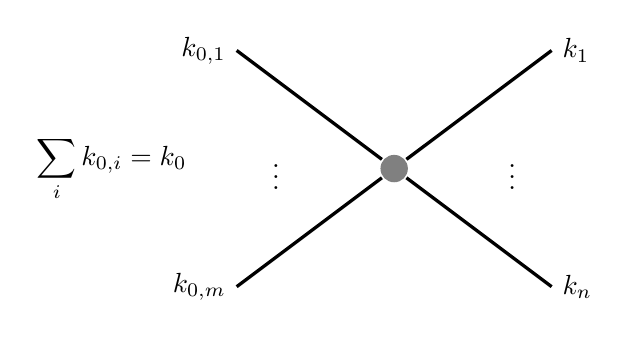
\begin{tikzpicture}[very thick]
    % 中心相互作用顶点 (灰色实心圆)
    \node[circle, fill=gray, inner sep=3.5pt] (v) at (0,0) {};
    
    % 左侧外腿 (无质量部分)
    \draw (v) -- (-2, 1.5) node[left] {$k_{0,1}$};
    \draw (v) -- (-2, -1.5) node[left] {$k_{0,m}$};
    
    % 左侧外腿之间的省略号
    \node at (-1.5, 0) {$\vdots$};
    
    % 左侧动量和的标记
    \node[left] at (-2.5, 0) {$\displaystyle \sum_i k_{0,i} = k_0$};
    
    % 右侧外腿（有质量部分）
    \draw (v) -- (2, 1.5) node[right] {$k_1$};
    \draw (v) -- (2, -1.5) node[right] {$k_n$};
    
    % 右侧外腿之间的省略号
    \node at (1.5, 0) {$\vdots$};
    
\end{tikzpicture}
\end{document}
